\documentclass[compress]{beamer}
\usecolortheme{default}

\usepackage{lmodern, epstopdf, multirow, array, setspace, bbm, tcolorbox, pbox, bm, mathtools, tikz}
\usepackage[T1]{fontenc}

\setbeamertemplate{frametitle}[default][center]
\setbeamertemplate{footline}{\hfill \insertframenumber/\inserttotalframenumber\hspace*{5pt}\vspace{5pt}}
\setbeamertemplate{navigation symbols}{}

\newlength{\wideitemsep}
\setlength{\wideitemsep}{\itemsep}
\addtolength{\wideitemsep}{4pt}
\let\olditem\item
\renewcommand{\item}{\setlength{\itemsep}{\wideitemsep}\olditem}
\setlength{\leftmargini}{12pt}
\setlength{\leftmarginii}{14pt}
\setbeamertemplate{itemize/enumerate subbody begin}{\vspace{6pt}}
\setbeamertemplate{itemize item}[circle]
\setbeamertemplate{enumerate item}[circle]
\setbeamertemplate{enumerate subitem}[default]

\setbeamercolor{alerted text}{fg=blue}
\setbeamersize{text margin left=1.5em,text margin right=1.5em}

\tcbset{
    colback=white,
    colframe=black,
    coltext=black,
    coltitle=blue,
    colbacktitle=white,
    boxrule=1pt,
    titlerule=0pt,
    toptitle=4pt,
    top=2pt
}

\newenvironment{changemargin}[2]{% 
  \begin{list}{}{% 
    \setlength{\topsep}{0pt}% 
    \setlength{\leftmargin}{#1}% 
    \setlength{\rightmargin}{#2}% 
    \setlength{\listparindent}{\parindent}% 
    \setlength{\itemindent}{\parindent}% 
    \setlength{\parsep}{\parskip}% 
  }% 
  \item[]}{\end{list}}
  
\newenvironment{defn}{%
  \begin{tcolorbox}[title={Definition}]%
  }{\end{tcolorbox}}
  
\newenvironment{prop}[1]{%
  \begin{tcolorbox}[title={Proposition #1}]%
  }{\end{tcolorbox}}
  
\newcommand{\cit}[1]{{\footnotesize \textcolor[rgb]{0.5,0,0}{#1}}}

% Font size for code listings (verbatim blocks); reset with \normalsize
\newcommand{\codesize}{\fontsize{7}{8.5}\selectfont}

\newcommand{\slidesetup}[1]{%
  \title{#1}%
  \subtitle{\texorpdfstring{\vspace{0.3\baselineskip}}{} {\small This version: \today}}%
  \author[Mikkel Plagborg-Moller]{ECMA 31150, Spring 2026 \texorpdfstring{\\[0.5ex]}{} University of Chicago \texorpdfstring{\\[0.5ex]}{} Department of Economics \texorpdfstring{\\[4ex]}{} Mikkel Plagborg-Moller}%
  \date{}%
}

% \circleoverlay[options]{text}
% Draws a red circle with a text box nearby on a tikz overlay.
% Options (with defaults):
%   cx=0cm, cy=0cm      - circle center (shift from page center)
%   r=1cm               - circle radius
%   tx=0cm, ty=0cm      - text box offset from circle center
%   text anchor=east    - anchor of text node (east = text left, west = text right)
%   font=\normalsize    - font size for text
\pgfkeys{
  /circleoverlay/.cd,
  cx/.store in=\cocx, cx=0cm,
  cy/.store in=\cocy, cy=0cm,
  r/.store in=\cor, r=1cm,
  tx/.store in=\cotx, tx=0cm,
  ty/.store in=\coty, ty=0cm,
  text anchor/.store in=\cotextanchor, text anchor=east,
  font/.store in=\cofont, font=\normalsize,
}
\newcommand{\circleoverlay}[2][]{%
  \pgfkeys{/circleoverlay/.cd, cx=0cm, cy=0cm, r=1cm, tx=0cm, ty=0cm, text anchor=east, font=\normalsize, #1}%
  \pgfmathsetlengthmacro{\circlediameter}{2*\cor}%
  \node[draw=red, line width=2pt, circle, minimum size=\circlediameter, inner sep=0pt]
    (tmpcirc) at ([xshift=\cocx,yshift=\cocy]current page.center) {};%
  \node[anchor=\cotextanchor, fill=white, draw=red, text=red, inner sep=4pt, align=left, font=\cofont]
    at ([xshift=\cotx,yshift=\coty]tmpcirc.center) {#2};%
}

\DeclareMathOperator*{\argmax}{argmax}
\DeclareMathOperator*{\argmin}{argmin}
\DeclareMathOperator{\diag}{diag}
\DeclareMathOperator{\var}{Var}
\DeclareMathOperator{\cov}{Cov}
\DeclareMathOperator{\corr}{Corr}
\DeclareMathOperator{\lrv}{LRV}


\slidesetup{State space models II}

\begin{document}
\frame{
\maketitle
}

\frame{
\frametitle{Plan for this slide deck}
\begin{enumerate}
\item Modeling time-varying parameters
\item Missing data
\item Mixed-frequency data, nowcasting
\item High-dimensional factor models
\item Models with regime switching
\end{enumerate}
}

\frame{
\frametitle{State space model with time-varying coefficients}
\begin{itemize}
\item Consider a state space model where the coefficients depend on time:
\begin{align*}
\bm{y}_t &= \bm{c}_{\alert{t}} + \bm{G}_{\alert{t}}\bm{s}_t + \bm{v}_t, \\
\bm{s}_t &= \bm{F}_{\alert{t}}\bm{s}_{t-1} + \bm{u}_t, \\
\begin{pmatrix}
\bm{v}_t \\
\bm{u}_t
\end{pmatrix} &\overset{indep}{\sim} N\left(\bm{0}, \begin{pmatrix}
\bm{V}_{\alert{t}} & \bm{0} \\
\bm{0} & \bm{U}_{\alert{t}}
\end{pmatrix} \right).
\end{align*}
\item Implicit assumption: whatever is driving the time-variation in the coefficients is only related to the conditional variances of the shocks, not their conditional means.
\begin{itemize}
\item Rules out that $\bm{u}_t$ is directly affecting the path for $\bm{G}_t$, say.
\end{itemize}
\item The Kalman filter and smoother algorithms apply exactly as in the last slide deck. We just need to put time subscripts on all the coefficient vectors/matrices: $\bm{c} \rightarrow \bm{c}_t$, $\bm{G} \rightarrow \bm{G}_t$, etc.
\begin{itemize}
\item Smoother algorithm: when defining $\bm{J}_t$, substitute $\bm{F} \rightarrow \bm{F}_{t+1}$.
\end{itemize}
\end{itemize}
}

\frame{
\frametitle{Example: time-varying parameters}
\begin{itemize}
\item Economic relationships may change over time.
\item Consider a time series regression model with time-varying slope:
\begin{align*}
y_t &= \alert{\beta_t} x_t + v_t, \\
\beta_t &= \beta_{t-1} + u_t, \\
\begin{pmatrix}
v_t \\
u_t
\end{pmatrix} &\overset{iid}{\sim} N\left(\begin{pmatrix}
0 \\
0
\end{pmatrix}, \begin{pmatrix}
\sigma_v^2 & 0 \\
0 & \sigma_u^2
\end{pmatrix}\right).
\end{align*}
\item Fits into the framework on the previous slide:
\[\bm{s}_t \equiv \beta_t,\quad \bm{c}_t\equiv 0,\quad \bm{G}_t \equiv x_t, \quad \bm{F}_t \equiv 1,\quad \bm{V}_t \equiv \sigma_v^2,\quad \bm{U}_t \equiv \sigma_u^2.\]
\item Note: we're assuming that $\lbrace x_t \rbrace$ is independent of the shocks $\lbrace u_t,v_t \rbrace$.
\item \alert{Exercise:} propose a more general state space model where the regression residual is serially correlated (e.g., an AR(1) process).
\end{itemize}
}

\begin{frame}[fragile]
\tiny
\begin{verbatim}
def kalman_filter(Y, c, G, V, F, U, s0, P0):
    T, n = Y.shape
    m = F.shape[-1]

    s_pred = np.zeros((T, m))       # s_{t|t-1}
    P_pred = np.zeros((T, m, m))    # P_{t|t-1}
    s_filt = np.zeros((T, m))       # s_{t|t}
    P_filt = np.zeros((T, m, m))    # P_{t|t}
    y_pred = np.zeros((T, n))       # y_{t|t-1}
    Q_pred = np.zeros((T, n, n))    # Q_{t|t-1}

    s_prev, P_prev = s0, P0
    for t in range(T):
        # Predict
        s_pred[t] = F[t] @ s_prev
        P_pred[t] = F[t] @ P_prev @ F[t].T + U[t]
        y_pred[t] = c[t] + G[t] @ s_pred[t]
        Q_pred[t] = G[t] @ P_pred[t] @ G[t].T + V[t]

        # Gain
        K = np.linalg.solve(Q_pred[t], G[t] @ P_pred[t]).T

        # Update
        innov = Y[t] - y_pred[t]
        s_filt[t] = s_pred[t] + K @ innov
        P_filt[t] = P_pred[t] - K @ Q_pred[t] @ K.T

        s_prev, P_prev = s_filt[t], P_filt[t]

    return {'s_pred': s_pred, 'P_pred': P_pred,
            's_filt': s_filt, 'P_filt': P_filt,
            'y_pred': y_pred, 'Q_pred': Q_pred}
\end{verbatim}
\end{frame}

\begin{frame}[fragile]
\tiny
\begin{verbatim}
def kalman_smoother(filt, F):
    s_pred, P_pred = filt['s_pred'], filt['P_pred']
    s_filt, P_filt = filt['s_filt'], filt['P_filt']
    T, m = s_filt.shape

    s_smooth = np.zeros((T, m))     # s_{t|T}
    P_smooth = np.zeros((T, m, m))  # P_{t|T}

    # Initialize at final filtered state
    s_smooth[T - 1] = s_filt[T - 1]
    P_smooth[T - 1] = P_filt[T - 1]
    
    for t in range(T - 2, -1, -1):
        J = np.linalg.solve(P_pred[t + 1], F[t + 1] @ P_filt[t]).T
        s_smooth[t] = s_filt[t] + J @ (s_smooth[t + 1] - s_pred[t + 1])
        P_smooth[t] = P_filt[t] + J @ (P_smooth[t + 1] - P_pred[t + 1]) @ J.T

    return {'s_smooth': s_smooth, 'P_smooth': P_smooth}
\end{verbatim}
\end{frame}

\frame{
\begin{figure}
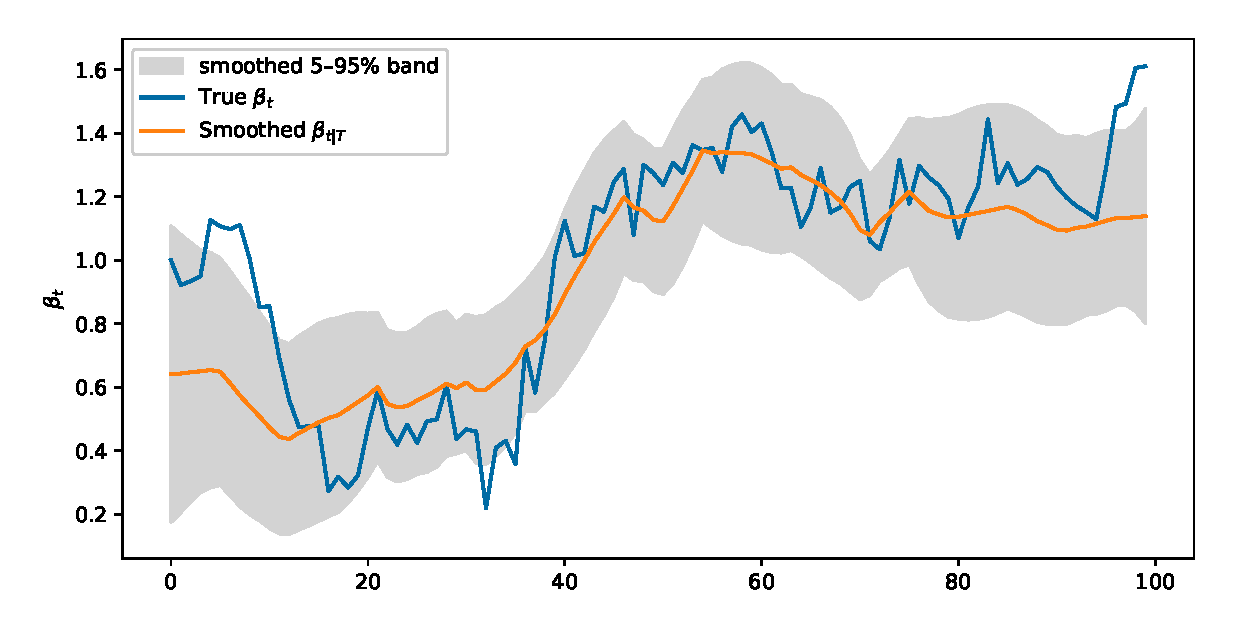
\includegraphics[width=\linewidth]{fig/tvp.eps} \\
\vspace{-\baselineskip}
\[y_t = \beta_t x_t + v_t, \quad \beta_t = \beta_{t-1} + u_t,\quad \beta_0=1\]
\[\sigma_u=0.1,\quad \sigma_v=0.5,\quad T=100\]
\[x_t \sim \text{AR(1) with } \rho=0.7 \text{ and } \var(x_t) = 1\]
\end{figure}
}

\frame{
\frametitle{Missing data}
\begin{itemize}
\item State space models are great at dealing with missing data.
\item Consider a constant-coefficient state space model:
\begin{align*}
\bm{y}_t &= \bm{c} + \bm{G}\bm{s}_t + \bm{v}_t,\quad \bm{v}_t \overset{iid}{\sim} N(\bm{0},\bm{V}), \\
\bm{s}_t &= \bm{F}\bm{s}_{t-1} + \bm{u}_t,\quad \bm{u}_t \overset{iid}{\sim} N(\bm{0},\bm{U}).
\end{align*}
\item But suppose that at some time points $t \in \mathcal{T}_\text{missing}$, the first variable $y_{1t}$ is \textbf{missing}: we only observe $y_{2t},\dots,y_{nt}$ at these points in time.
\item We will see that a model with time-varying coefficients can capture the missing data.
\end{itemize}
}

\frame{
\begin{figure}
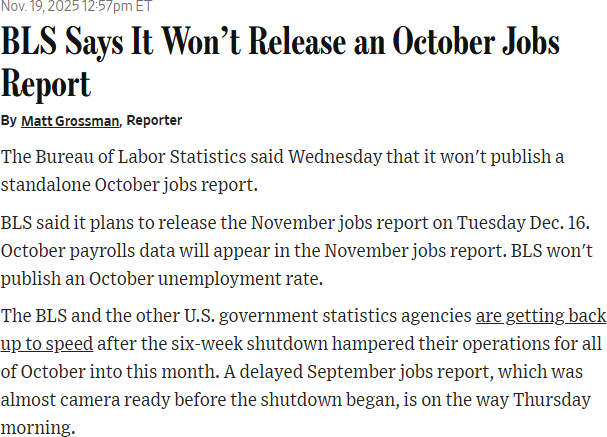
\includegraphics[width=0.8\linewidth]{fig/shutdown.png} \\
\bigskip\bigskip
\tiny
\url{https://www.wsj.com/economy/bls-wont-publish-october-inflation-report-dcf45b03}
\end{figure}
}

\frame{
\frametitle{Missing data: state space model}
\begin{itemize}
\item Define
\[\bm{c}_t \equiv \begin{cases}
\bm{c} & \text{for } t \notin \mathcal{T}_\text{missing}, \\
\bm{c} \text{ with first element replaced by zero} & \text{for } t \in \mathcal{T}_\text{missing},
\end{cases}\]
\[\bm{G}_t \equiv \begin{cases}
\bm{G} & \text{for } t \notin \mathcal{T}_\text{missing}, \\
\bm{G} \text{ with first row replaced by zeros} & \text{for } t \in \mathcal{T}_\text{missing},
\end{cases}\]
\[\bm{V}_t \equiv \begin{cases}
\bm{V} & \text{for } t \notin \mathcal{T}_\text{missing}, \\
\begin{pmatrix}
\omega^2 & \bm{0}_{1 \times (n-1)} \\
\bm{0}_{(n-1) \times 1} & \bm{V}_{2:,2:}
\end{pmatrix} & \text{for } t \in \mathcal{T}_\text{missing},
\end{cases}\]
where $\bm{V}_{2:,2:}$ contains rows 2--$n$ and columns 2--$n$ of $\bm{V}$, and $\omega^2$ is an arbitrary number.
\item Then consider the state space model with time-varying coefficients
\begin{align*}
\bm{y}_t &= \alert{\bm{c}_t} + \alert{\bm{G}_t}\bm{s}_t + \bm{v}_t, \quad \bm{v}_t \sim N(\bm{0},\alert{\bm{V}_t}), \\
\bm{s}_t &= \bm{F}\bm{s}_{t-1} + \bm{u}_t,\quad \bm{u}_t \sim N(\bm{0},\bm{U}).
\end{align*}
\end{itemize}
}

\frame{
\frametitle{Missing data: state space model (cont.)}
\begin{align*}
\bm{y}_t &= \alert{\bm{c}_t} + \alert{\bm{G}_t}\bm{s}_t + \bm{v}_t, \quad \bm{v}_t \sim N(\bm{0},\alert{\bm{V}_t}), \\
\bm{s}_t &= \bm{F}\bm{s}_{t-1} + \bm{u}_t,\quad \bm{u}_t \sim N(\bm{0},\bm{U})
\end{align*}
\vspace{-0.5\baselineskip}
\begin{itemize}
\item At dates $t \notin \mathcal{T}_\text{missing}$, the model has $\bm{c}_t=\bm{c}$, $\bm{G}_t=\bm{G}$, $\bm{V}_t=\bm{V}$.
\item At dates $t \in \mathcal{T}_\text{missing}$, the observation equation for $y_{1t}$ becomes
\[y_{1t} = v_{1t},\quad v_{1t} \sim N(0,\omega^2), \quad v_{1t} \text{ is independent of } (v_{2t},\dots,v_{nt}).\]
Therefore, $y_{1t}$ is independent of $\bm{s}_t$ and of $(y_{2t},\dots,y_{nt})$.
\end{itemize}
}

\frame{
\frametitle{Missing data: filter and smoother}
\begin{itemize}
\item Consider running the Kalman filter/smoother for the model with time-varying coefficients on the previous slide.
\item Feed in any arbitrary ``data'' $y_{1t}$ when it's missing. For example, just set $y_{1t} \equiv 0$ for $t \in \mathcal{T}_\text{missing}$.
\item By design, the filter/smoother won't use the fake data $\lbrace y_{1t} \rbrace_{t \in \mathcal{T}_\text{missing}}$ to infer $\bm{s}_t$ or to contribute to the likelihood for any parameters.
\item But $\bm{s}_{t|t}$ and the likelihood contribution are still optimally computed based on the available real data $(y_{2t},\dots,y_{nt})$ also for $t \in \mathcal{T}_\text{missing}$.
\item \alert{Exercise:} how can you generalize the procedure to allow multiple time series to be missing?
\end{itemize}
}

\frame{
\begin{figure}
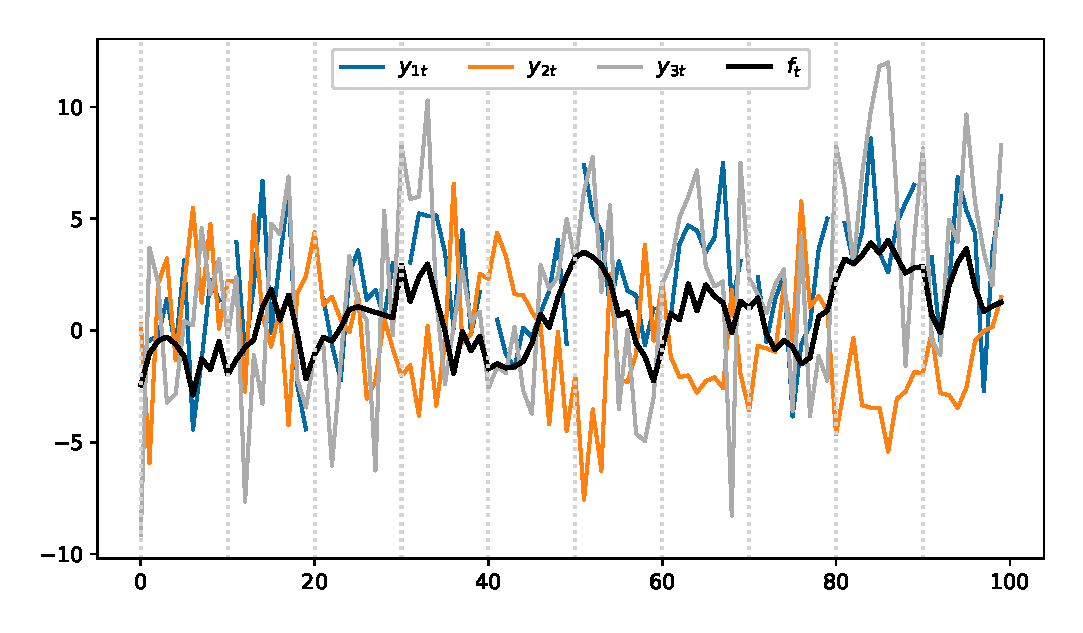
\includegraphics[width=\linewidth]{fig/factor_sim_missing.eps} \\
\medskip
Simulation: same dynamic factor model as in previous slide deck, \\
but $y_{1t}$ is missing every 10 periods.
\end{figure}
}

\frame{
\begin{figure}
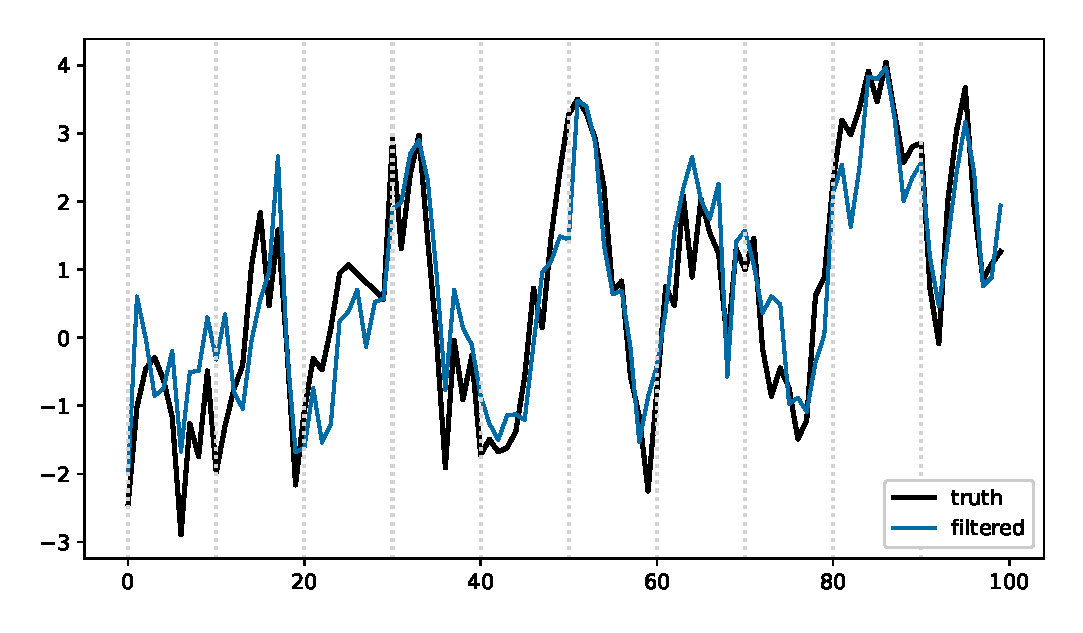
\includegraphics[width=\linewidth]{fig/factor_filter_missing.eps} \\
\medskip
Note: filtered state $s_{t|t}$ is updated also on dates where $y_{1t}$ is missing, using info from $(y_{2t},y_{3t})$ and from dynamic model for $s_t$.
\end{figure}
}

\frame{
\frametitle{Mixed-frequency data}
\begin{itemize}
\item A special case of missing data is when we observe time series at multiple frequencies, e.g., monthly and quarterly.
\item Can specify a state space model where latent state vector is defined at highest frequency. Low-frequency data is missing in the observation equation in between low-frequency data points.
\item Example:
\begin{itemize}
\item Have data on monthly industrial production (IP) and quarterly GDP.
\item State $s_t$: latent measure of real total output, monthly.
\item IP enters in observation equation every period.
\item GDP only enters observation equation in March, June, September, December, and is related to $s_t + s_{t-1} + s_{t-2}$.
\end{itemize}
\end{itemize}
}

\frame{
\frametitle{Mixed-frequency data: nowcasting}
\begin{itemize}
\item \textbf{Nowcasting} is the act of forecasting the data (e.g., GDP) that applies to the \emph{current} time period \emph{before} the statistical agency actually releases said data.
\item We would like to condition the nowcast on a diverse mix of leading indicators measured at various high frequencies, in addition to lower-frequency data (e.g., lagged GDP).
\item Data is released by different statistical agencies on different schedules.
\item Massive missing data problem at the end of the sample!
\item The New York Fed's nowcast model is a sophisticated dynamic factor model that handles the missing/mixed-frequency data.
\begin{itemize}
\item See Bok et al.\ (2018) and Almuzara et al.\ (2023) on the reading list.
\end{itemize}
\end{itemize}
}

\frame{
\begin{figure}
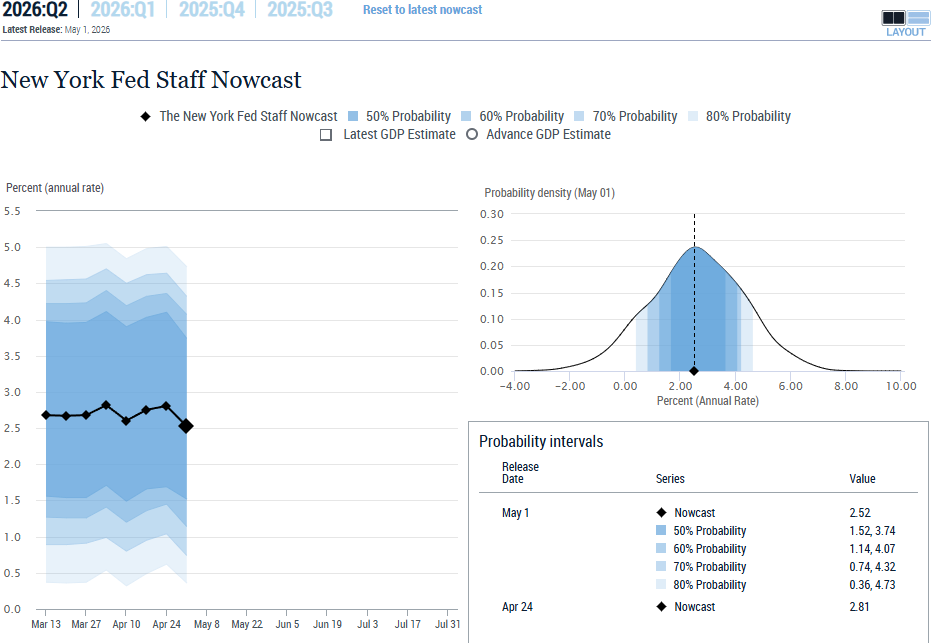
\includegraphics[width=0.9\linewidth]{fig/nyfed_nowcast1.png} \\
\medskip
\url{https://www.newyorkfed.org/research/policy/nowcast}
\end{figure}
}

\frame{
\begin{figure}
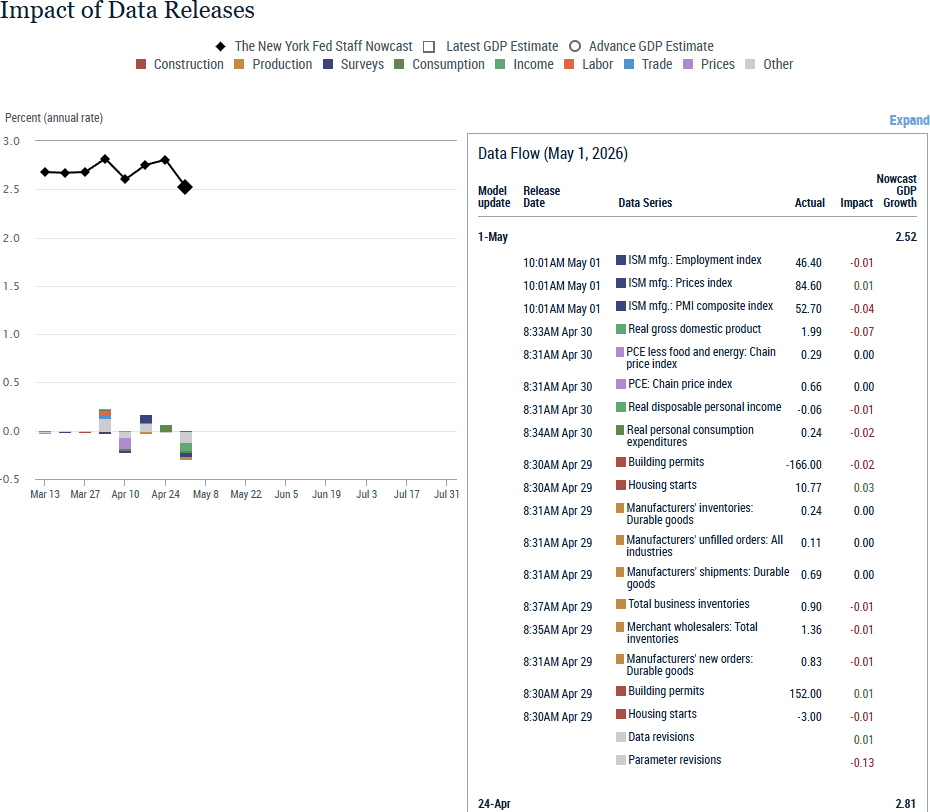
\includegraphics[width=0.8\linewidth]{fig/nyfed_nowcast2.png}
\end{figure}
}

\frame{
\frametitle{High-dimensional factor models}
\begin{itemize}
\item Consider a dynamic factor model with multiple latent factors and their lags:
\[\bm{y}_t = \bm{c} + \bm{\lambda}_0 \bm{f}_t + \bm{\lambda}_1 \bm{f}_{t-1} + \dots + \bm{\lambda}_p \bm{f}_{t-p} + \bm{v}_t.\]
\item We assume the dimension $r$ of the latent factors $\bm{f}_t$ is relatively small.
\item But suppose we want to condition our analysis on a large number $n$ of observed variables $\bm{y}_t = (y_{1t},\dots,y_{nt})'$.
\begin{itemize}
\item E.g., data for many sectors/countries.
\end{itemize}
\item We could treat this as a state space model and do Bayesian inference via the Kalman filter likelihood. However, this could be computationally tricky when $n$ is large.
\end{itemize}
}

\frame{
\frametitle{High-dimensional factor models: PCA}
\[\bm{y}_t = \bm{c} + \bm{\lambda}_0 \bm{f}_t + \dots + \bm{\lambda}_p \bm{f}_{t-p} + \bm{v}_t.\]
\vspace{-0.5\baselineskip}
\begin{itemize}
\item Turns out we can consistently estimate the factors $\bm{f}_t$ and loadings $\bm{\lambda}_j$ (up to some normalizations) using the technique of \textbf{principal component analysis} (PCA).
\item This involves computing eigenvectors of the $n \times n$ sample variance-{\allowbreak}covariance matrix of the data $\bm{y}_t$. Computationally very simple!
\begin{itemize}
\item The PCA estimates could be used as a starting point for subsequent Bayesian inference using state space methods.
\end{itemize}
\item Details: Stock \& Watson (2019) textbook, chapter 17.6; Stock \& Watson (2016) handbook chapter (on syllabus).
\item High-dimensional factor models are some of the most empirically successful economic forecasting models.
\end{itemize}
}

\frame{
\frametitle{Regime switching}
\begin{itemize}
\item In the linear-Gaussian state space model, the latent state vector $\bm{s}_t$ is normally distributed.
\item In some applications, it makes more sense to think of a \emph{discrete} latent state, also known as a \textbf{regime} (e.g., recession vs.\ expansion).
\end{itemize}
}

\frame{
\frametitle{Regime switching: example}
\begin{itemize}
\item Regime-switching AR(1) model:
\[y_t = \begin{cases}
c_1 + \rho_1 y_{t-1} + u_t,\quad u_t \sim N(0,\sigma_1^2) & \text{when } s_t=1, \\
c_2 + \rho_2 y_{t-1} + u_t,\quad u_t \sim N(0,\sigma_2^2) & \text{when } s_t=2.
\end{cases}\]
\item The latent regime $s_t \in \lbrace 1,2 \rbrace$ follows a discrete Markov chain:
\[P(s_t=i \mid s_{t-1}=j,\lbrace y_{t-\ell},s_{t-1-\ell}\rbrace_{\ell \geq 1}) = P(s_t=i \mid s_{t-1}=j) \equiv \Pi_{ij},\]
where $\Pi_{ij}$ are the \textbf{transition probabilities}.
\item The AR dynamics depend on the regime. The regime switches occasionally according to the transition probabilities.
\end{itemize}
}

\frame{
\begin{figure}
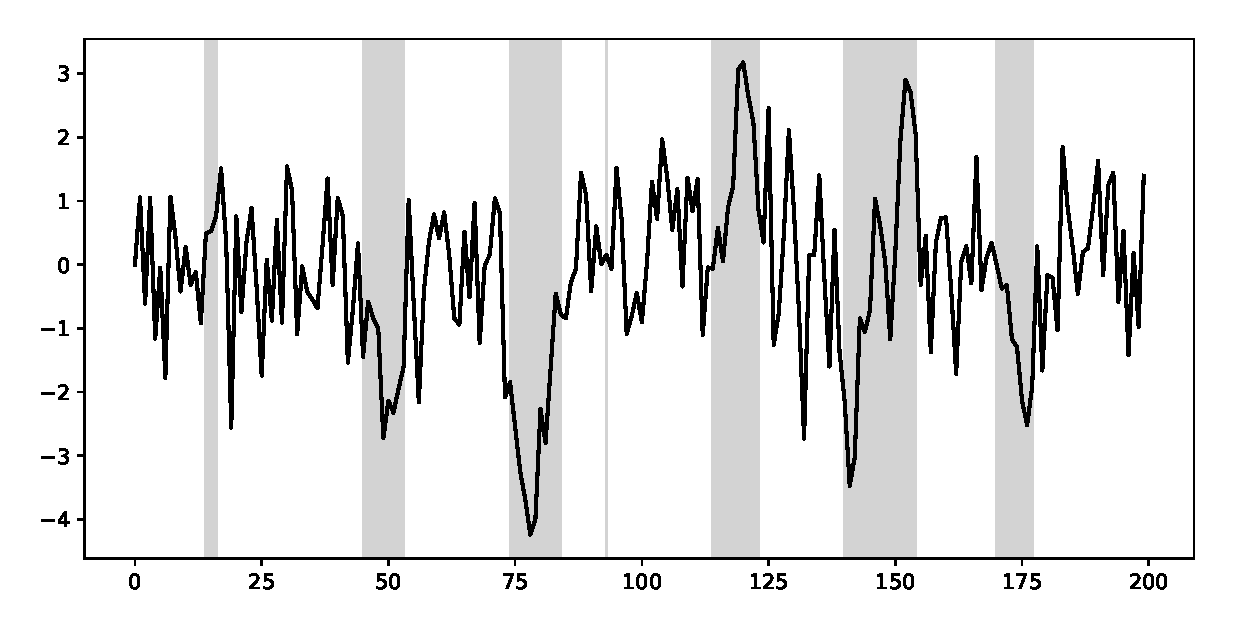
\includegraphics[width=\linewidth]{fig/regime_switching.eps} \\
\medskip
Simulated regime-switching AR(1) model \\
\smallskip
Regime 1: $\rho_1=0$, regime 2 (in gray): $\rho_2=0.9$ \\
\smallskip
Regime $s_t$ switches with probability 0.1 every period \\
\end{figure}
}

\frame{
\frametitle{Regime switching: filtering and smoothing}
\begin{itemize}
\item There exist analogues of the Kalman filter and smoother for models with discrete latent regimes.
\begin{itemize}
\item Can be applied to much more general models than the example on the previous slide.
\end{itemize}
\item The filtering algorithm also produces the likelihood function, so we can do Bayesian inference on the parameters.
\item See Hamilton (1994) textbook, chapter 22.
\end{itemize}
}

\frame{
\frametitle{Further reading (on syllabus)}
\begin{itemize}
\item More examples of state space models + computational tricks:
\begin{itemize}
\item Durbin \& Koopman (2012) book.
\item Brockwell \& Davis (2016) textbook, chapter 9.
\end{itemize}
\item How to use state space techniques to estimate structural macro models:
\begin{itemize}
\item Herbst \& Schorfheide (2015) book.
\item Mancini Griffoli (2013) user guide for Dynare software package.
\end{itemize}
\end{itemize}
}

\frame{
\frametitle{What did we learn?}
\begin{itemize}
\item State space model with time-varying coefficients
\begin{itemize}
\item Time-varying parameter models
\item Missing data
\item Mixed-frequency data, nowcasting
\end{itemize}
\item High-dimensional factor models
\item Discrete regime switching
\end{itemize}
}

\frame{
\frametitle{Looking ahead}
\begin{itemize}
\item How can we model data that is not stationary?
\item How do our usual statistical procedures (e.g., regression) perform when we apply them to non-stationary data?
\item How can we test the stationarity assumption?
\end{itemize}
}

\end{document}